%ARC --> 3 cartes de Dobble  Blocking set:2 tas
\documentclass[a4paper]{article}

\title{Rapport de stage}
\usepackage[utf8]{inputenc}
\usepackage[francais]{babel}
\usepackage{amsmath}
\usepackage{eufrak}
\usepackage{tikz}
\usepackage{graphicx}
\usepackage{listings}
\usepackage{verbatim}
\usepackage{sagetex}
\usepackage{array,multirow,makecell}
\usepackage{amssymb}
\usepackage[margin=3cm]{geometry}

\newtheorem{Def}{Définition}[section]
\newtheorem{Prop}[Def]{Proposition}
\newtheorem{Th}[Def]{Théorème}
\lstset{language=Python}
\usepackage{fancyhdr}
\pagestyle{fancy}
\begin{document}
\thispagestyle{empty}
\begin{center}

\centering

\vspace{3cm}

{\Huge Rapport de stage \ldots} \\ \vspace{0.3cm}
{\large Quentin Honoré}

\vspace{2cm}

\begin{tikzpicture}

\coordinate (P7) at (-7,0);
\coordinate (P5) at (7,0);
\coordinate (P1) at (0,18);
\coordinate (P6) at (barycentric cs:P5=1,P7=1);
\coordinate (P3) at (barycentric cs:P1=1.2,P7=1);
\coordinate (P2) at (barycentric cs:P1=1.2,P5=1);
\coordinate (P4) at (barycentric cs:P6=2,P1=1);

\draw[thick] (P1) -- (P7) -- (P5) -- cycle;
\draw[thick] (P3) -- (P5);
\draw[thick] (P1) -- (P6);
\draw[thick] (P2) -- (P7);

\draw[thick] (P3) .. controls (-3,2) .. (P6) .. controls (3,2) .. (P2) .. controls (0,12) .. (P3);

\foreach \x in {1,2,3,4,5,6,7}
  \node at (P\x) {\includegraphics[scale=0.3]{dobble\x.png}};
\end{tikzpicture}
\end{center}
\newpage
\tableofcontents
\newpage
\section*{Remerciements}
En premier lieu, je tiens à remercier mon maître de stage, Mr Vincent DELECROIX pour m'avoir accueilli chaleureusement, accompagné et aidé au cours de ces 8 semaines de stage. Je lui suis reconnaissant pour le temps qu'il m'a consacré.\\
Je remercie mon tuteur, Mr Jai pour le suivi tout au long de mon stage.\\

\newpage
\section*{Introduction}
Ce rapport est consacré au stage que j'ai effectué dans le cadre de ma formation à la Prépa des INP. Je devais effectuer un stage d'une durée minimale de 6 semaines afin de découvrir les métiers correspondant à ma formation.
J'ai donc fait mon stage au LaBRI, Laboratoire de Recherche Informatique à Bordeaux, du 4 Mai au 26 Juin où l'on m'a proposé un stage avec pour sujet ``\textit{Les designs combinatoires et le logiciel Sage}''.\vspace{1\baselineskip}\\
Ce stage m'a permis de mettre en pratique les connaissances acquises pendant les cours d'Informatique à la Prépa des INP, le logiciel Sage étant basé sur le langage de programmation Python. Il m'a permis d'acquérir de nouvelles compétences sur la programmation en Python, les méthodes de développement d'un logiciel open source avec par exemple le logiciel git et sur la rédaction des textes (y compris ce rapport) avec LaTEX.\vspace{1\baselineskip}\\
Au cours de ce stage j'ai pu découvrir les métiers de la recherche et le fonctionnement d'un laboratoire de recherche en Informatique. Il m'a conforté dans mon choix de l'Enseirb-Matmeca en filière Informatique comme école d'ingénieur et me fait réfléchir à une possible continuation sur un doctorat pour ensuite travailler dans la recherche.\vspace{1\baselineskip}\\
L'objectif de ce stage était de se familiariser avec les designs combinatoires et découvrir le fonctionnement du logiciel Sage et son développement afin d'implémenter certaines de ces constructions dans ce logiciel. \\
Dans ce rapport, je présenterais dans une première partie le LaBRI et ce qu'il s'y passe, puis j'aborderais tous les concepts mathématiques sur lesquels j'ai travaillé nécessaires à la compréhension de mes travaux, et enfin je présenterais Sage et les travaux que j'ai fait sur ce logiciel. 
\newpage
\section{Présentation du LaBRI}
Le LaBRI est une unité de recherche associée à Bordeaux INP, à l'université de Bordeaux et au CNRS et depuis 2002 partenaire de l'Inria (Institut national de recherche en informatique et en automatique). Il y a aujourd'hui au LaBRI environ 320 personnes dont 113 enseignant-e-s chercheu-r-ses, 37 chercheu-r-ses, 22 personnels administratifs et plus de 140 contractuels (doctorant-e-s, ingénieur-e-s).\vspace{1\baselineskip}\\
Six grandes équipes composent le laboratoire:
\begin{itemize}
\item Combinatoire et Algorithmique
  \begin{itemize}
  \item Combinatoire énumérative et algébrique
  \item Graphes et applications
  \item Algorithmique distribuée
    \end{itemize}
\item Image et Son
\item Méthodes Formelles
\item Modèles et Algorithmes pour la Bioinformatique et la Visualisation d'informations
\item Programmation, Réseaux et Systèmes
\item Supports et Algorithmes pour les applications numériques hautes performances
  \end{itemize}
\newpage
\section{Les plans projectifs finis}
\subsection{Définitions}
\begin{Def}
Soit P un ensemble fini (appelé points) et D un sous ensemble des parties de P (appelé droites). \\
On dit que le couple (P,D) est un plan projectif fini si et seulement si: \\
$\cdot$ Par deux points distincts passe une unique droite. \\
$\cdot$ Deux droites distinctes se coupent en un unique point. \\
$\cdot$ Il existe un quadrilatère (4 points tels que pour chaque triplet, les 3 points ne sont pas alignés).
\end{Def}
\textbf{Remarque}\\
  $\cdot$ Les 2 premières propositions sont symétriques. \\
$\cdot$ Un plan projectif est une structure d'incidence (un ensemble de points et un ensemble de droites).\vspace{1\baselineskip}\\
\textbf{Exemple}\\
On va construire un plan projectif fini d'ordre 2 (3 points par droite, et 3 droites se coupent en chaque point). On construit d'abord un quadrilatère. Dans cette géométrie, deux droites qui n'ont pas de points en commun sont dites parallèles. Les diagonales, les deux droites horizontales et les deux verticales \vspace{1\baselineskip}sont donc parallèles.\\
  Pourtant il nous faut bien une intersection pour tout couple de droites. On définit alors les intersections dites ``à l'infini'', c'est l'idée de base de la géométrie projective. De la même manière que pour le point de fuite chez les peintres, on dit que deux droites parallèles s'intersectent à l'infini. Imaginez vous sur une route, les deux bordures sont bien parallèles mais en regardant au loin, nous avons l'impression que la route se rétrécit pour ne devenir\vspace{1\baselineskip} qu'un point.\\
La première propriété nous dit maintenant que pour chaque couple de points, on a une unique droite. Nous allons donc construire la ``droite à l'infini'' qui passe par les points à l'infini (comme l'horizon dans la vie courante).
\begin{center}
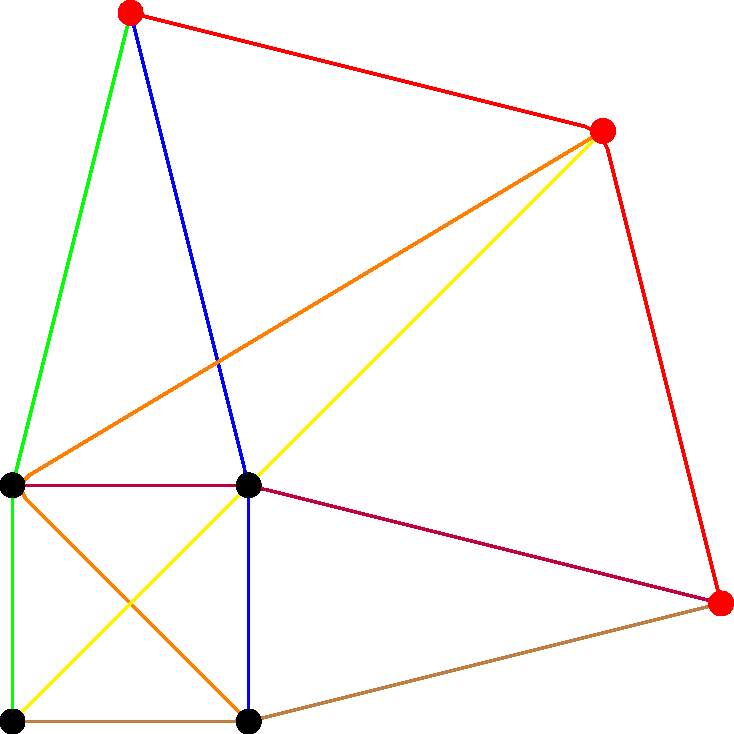
\includegraphics[scale=0.5]{test_tikz.pdf}
\end{center}
\vspace{2\baselineskip}
Les 3 propositions sont bien vérifiées.
\vspace{2\baselineskip}
\begin{Prop}
Toutes les droites contiennent le même nombre de points. Par symétrie, par tout point passe le même nombre de droites. Soit k+1 ($k\geq2$) ce nombre alors:
\begin{center}
$card(D)=card(P)=k^2+k+1$
\end{center}
\end{Prop}

\vspace{2\baselineskip}

En effet, si on considère un point P, k+1 droites passent par ce point. Sur chacune de ces droites, il y a k+1 points, donc k si on ne compte pas le point P. On a donc k(k+1) points en plus du point P, soit:
\begin{center}
$card(P)=k(k+1)+1=k^2+k+1$
\end{center}
\vspace{1\baselineskip}
\textbf{Remarque}\\
$\cdot$On ne peut pas avoir de plan projectif de cardinal 6,8,9,10,11,12,14...: \\
$2^2+2+1=7$ \\
  $3^2+3+1=13$\\

\begin{Def}{Arc} \\
  Un $k$-arc dans un plan projectif est un ensemble de $k$ points tel que pour tout triplet dans cet ensemble, les 3 points ne soient pas alignés.
\end{Def}
\vspace{1\baselineskip}
\begin{Def}{Blocking set}\\
 $\cdot$ Un \textit{blocking set} est un ensemble de points dans un plan projectif que chaque ligne intersecte mais qui ne contient pas une ligne entière.\\
  $\cdot$ Un \textit{blocking set} B est minimal si par chaque point P de B, une seule ligne intersecte B en P.\\
  $\cdot$ Un \textit{blocking set} de plus petite cardinalité est appelé \textit{committee}.\\
 $\cdot$  Les \textit{committee} sont des \textit{minimal blocking set}.
\end{Def}
\vspace{1\baselineskip}
\begin{Prop}{Propriété de Desargues}\\
  Soit deux triangles (non plats) ABC et A'B'C' de sommets deux à deux distincts (A de A', B de B' et C de C'). \\
  Les 3 droites (AA'), (BB') et (CC') sont concourantes (en un point S) \textbf{si et seulement si} les 3 points $P = (BC) \cap (B'C')$, $Q = (AC) \cap (A'C')$ et $R = (AB) \cap (A'B')$ sont alignés (sur une droite d)
  \end{Prop}
\begin{center}
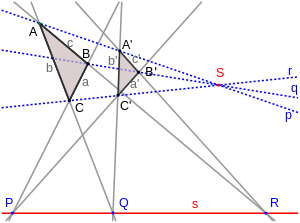
\includegraphics[scale=0.6]{desargues.png}  
\end{center}
\vspace{1\baselineskip}
\textbf{Remarque}\\
Cette propriété est connue sous le nom de théorème de Desargues dans les plans euclidiens. Dans les plans projectifs, la propriété n'est pas toujours vérifiée  
\newpage
\subsection{Le jeu du Dobble}
Le jeu du Dobble est un bon exemple de plan projectif fini. Si vous ne le connaissez pas, le Dobble est un jeu composé de 55 cartes sur lesquelles sont dessinés 8 symboles\vspace{1\baselineskip} différents.\\
  A chaque tour, pour gagner, il faut reconnaître le plus rapidement quel est le symbole commun entre sa propre carte et celle au milieu. Le jeu ne serait alors pas juste si l'un-e des joueu-r-ses avait deux symboles en commun avec la carte du milieu tandis que l'autre n'en\vspace{1\baselineskip} a aucun. \\
  Ces cartes sont donc construites de telle manière que pour toute paire de carte, il y ait un et un seul symbole en commun. On peut voir le Dobble comme un plan projectif en prenant pour droites les cartes et pour points les symboles mais aussi inversement en prenant pour points les cartes et pour droites les symboles.\vspace{1\baselineskip}\\
\begin{center}
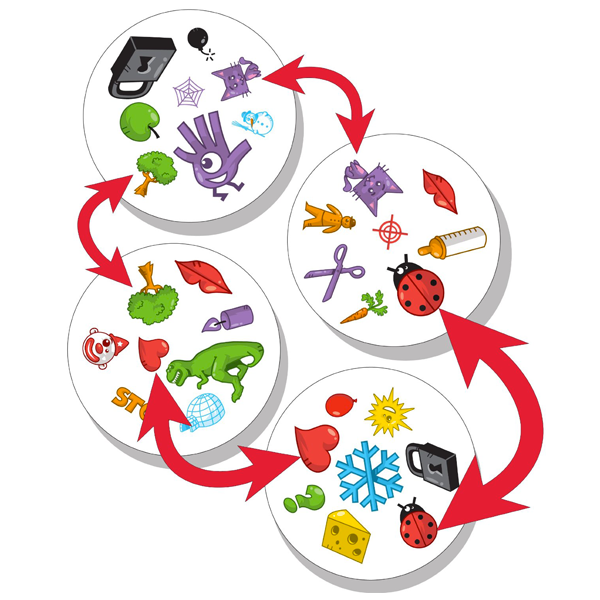
\includegraphics[scale=0.3]{dobble-2.jpg}
\end{center}
Avec 8 symboles par carte, on a donc un plan projectif d'ordre 7. Or $7^2+7+1=57$, il manque donc 2 cartes au Dobble. Si on étudie les cartes, on voit bien que le bonhomme de neige n'apparait que sur 6 cartes et quelques autres symboles sur 7 cartes. On arrive au même jeu si l'on construit nous même un plan projectif d'ordre 7 et qu'on retire 2 droites passant par un même point à la fin.\vspace{1\baselineskip}\\
En ajoutant ces deux cartes manquantes, le jeu du Dobble vérifie toutes les propriétés des plans projectifs. Néanmoins, même avec 2 cartes en moins, le Dobble garde sa propriété la plus importante: il y a toujours un unique symbole pour deux cartes même en enlevant 2 cartes.\vspace{1\baselineskip}\\
J'ai pu me procurer un jeu du Dobble. En numérotant les symboles (bonhomme orange $\rightarrow$ 0, bombe $\rightarrow$ 1, ..., igloo $\rightarrow$ 56), j'ai pu créer la liste des droites en ajoutant les 2 cartes manquantes.
\begin{sageverbatim}
  sage: blocks = [[6,11,21,27,43,50,53,55],[4,10,20,26,35,39,48,53],
        [8,10,28,31,34,45,54,55]], ... ,[0,46,48,34,32,27,52,14]]
\end{sageverbatim}
Après avoir importer la classe \textit{BalancedIncompleteBlockDesign}, on peut créer le plan projectif du Dobble.
\begin{sageverbatim}
 sage: from sage.combinat.designs.bibd import BalancedIncompleteBlockDesign
 sage: B=BalancedIncompleteBlockDesign(57,blocks)
 sage: B
 (57,8,1)-Balanced Incomplete Block Design
\end{sageverbatim}
Le Dobble est un plan projectif d'ordre 7 ($k+1=8$ et $k^2+k+1=57$).\\
\newpage
Je me suis alors servi d'un programme que j'avais précédemment fait pour les plans de Hughes. La fonction $is\_desarguesian\_plane$ itère sur les paires de triangles (non-plats) simplement pour vérifier que le théorème de Hughes. En pratique, si un plan n'est pas desarguesien, le programme affiche rapidement des centaines de paires de triangle pour lesquelles le théorème n'est pas vérifié et il n'est pas nécessaire de laisser tourner le programme plus longtemps.
\begin{sageverbatim}
 sage: is_desarguesian_plane(B)
 True
\end{sageverbatim}
Le Dobble(en ajoutant les cartes manquantes) est un plan projectif fini d'ordre 7 desarguesien. Il a donc été construit à partir du corps $\mathbb{F}_7$.
\vspace{2\baselineskip}\\
Le Dobble nous permet aussi de mieux comprendre les notions d'arc et de blocking set. Ici, les points sont les cartes et les droites sont les points.\vspace{2\baselineskip}\\
Si on prend un tas de cartes du Dobble, telles qu'il n'y ait pas plus de deux cartes contenant le même symbole, on a un arc. \\
Si on peut séparer le jeu du Dobble en deux tas tels que que tous les symboles soient représentés dans chacun des tas, on a un blocking set. En effet, pour chaque droite, on trouve au moins un point de chaque droite dans chacun des tas et puisqu'on en trouve au moins un dans l'autre tas aussi, aucun des 2 tas ne contient tous les points de la droite.
\newpage
\subsection{Les corps finis}
\begin{Def}
  Un corps fini est un corps commutatif qui est en plus fini.\\
  \begin{itemize}
\item il y a un élément neutre pour l'addition (noté $0$).
\item il y a un élément neutre pour la multiplication (noté $1$).
\item tous les éléments admettent un inverse pour l'addition.
\item tous les éléments différents de 0 ont un inverse pour la multiplication.
\item et certaines propriétés de commutativité, associativité qu'il n'est pas nécessaire de détailler ici.
  \end{itemize}
Un corps fini est uniquement défini par son cardinal qui doit être la puissance d'un nombre premier. On le note $\mathbb{F}_n$.
Si n est un nombre premier, alors $\mathbb{F}_n$ est $\mathbb{Z}/n\mathbb{Z}$.
\end{Def}
  Dans ce cas, on utilise la multiplication et l'addition usuelles congrues à $n$. Par exemple si on se place dans $\mathbb{F}_3$:\\
  $2*2=4$ et $4 \equiv 1 [3]$ donc dans $\mathbb{F}_3,2*2=1$\\
  De la même façon, $1+2=0$ sur $\mathbb{F}_3$\vspace{1\baselineskip}.\\
Il faut bien garder en tête que les éléments de ces corps finis n'ont que la notation en commun avec les entiers naturels que nous connaissons. L'élément que nous notons 2 dans $\mathbb{F}_3$ n'est pas l'entier 2.\vspace{1\baselineskip}\\
\textbf{Exemple}\\
  Par exemple, l'ensemble des réels est un corps tandis que l'ensemble des entiers naturels n'en est pas un : 2 n'admet pas d'inverse multiplicatif ni d'inverse additif.
\begin{center}
$\mathbb{F}_2 $\\
\begin{tabular}{|c|c|c|}
  \hline
  + & \textbf{0} & \textbf{1} \\
  \hline
  \textbf{0} & 0 & 1 \\
  \hline
  \textbf{1} & 1 & 0 \\
  \hline
\end{tabular}
\begin{tabular}{|c|c|c|}
  \hline
  $*$ & \textbf{0} & \textbf{1} \\
  \hline
  \textbf{0} & 0 & 0\\
  \hline
  \textbf{1} & 0 & 1\\
  \hline
\end{tabular}\\
\vspace{1\baselineskip}
$\mathbb{F}_3 $\\
\begin{tabular}{|c|c|c|c|}
  \hline
  + & \textbf{0} & \textbf{1} & \textbf{2} \\
  \hline
  \textbf{0} & 0 & 1 & 2 \\
  \hline
  \textbf{1} & 1 & 2 & 0 \\
  \hline
  \textbf{2} & 2 & 0 & 1 \\
  \hline
\end{tabular}
\begin{tabular}{|c|c|c|c|}
  \hline
  $*$ & \textbf{0} & \textbf{1} & \textbf{2} \\
  \hline
  \textbf{0} & 0 & 0 & 0 \\
  \hline
  \textbf{1} & 0 & 1 & 2 \\
  \hline
  \textbf{2} & 0 & 2 & 1 \\
  \hline
\end{tabular}\\
\vspace{1\baselineskip}
$\mathbb{F}_4$\\
\begin{tabular}{|c|c|c|c|c|}
  \hline
  + & \textbf{0} & \textbf{1} & \textbf{x} & \textbf{x+1} \\
  \hline
  \textbf{0} & 0 & 1 & x & x+1 \\
  \hline
  \textbf{1} & 1 & 0 & x+1 & x \\
  \hline
  \textbf{x} & x & x+1 & 0 & 1 \\
  \hline
  \textbf{x+1} & x+1 & x & 1 & 0 \\
  \hline
\end{tabular}
\begin{tabular}{|c|c|c|c|c|}
  \hline
  $*$ & \textbf{0} & \textbf{1} & \textbf{x} & \textbf{x+1} \\
  \hline
  \textbf{0} & 0 & 0 & 0 & 0 \\
  \hline
  \textbf{1} & 0 & 1 & x & x+1 \\
  \hline
  \textbf{x} & 0 & x & x+1 & 1 \\
  \hline
  \textbf{x+1} & 0 & x+1 & 1 & x\\
  \hline
\end{tabular}
\end{center}
\newpage

\subsection{Plan desarguesien}
On peut construire les plans desarguesiens à partir des corps finis. Comme leur nom l'indique, la propriété de Desargues est vérifiée sur ces plans.\\
Pour construire un plan à partir du corps $GF(q)$,\\
Nous allons donner aux points des coordonnées $(x,y,z)$ avec $x,y,z \in GF(q) et (x,y,z) \neq (0,0,0)$. Les points sont définis à multiplication près : pour $k \neq 0$, $k(x,y,z) = (kx,ky,kz) = (x,y,z)$.\\
Ici aussi, comme pour les plans euclidiens, les droites ont une équation de la forme $ax + by + cz = 0$ avec $(a,b,c) \neq (0,0,0)$. Les droites correspondantes seront notées $(a,b,c)$.
\begin{center}
  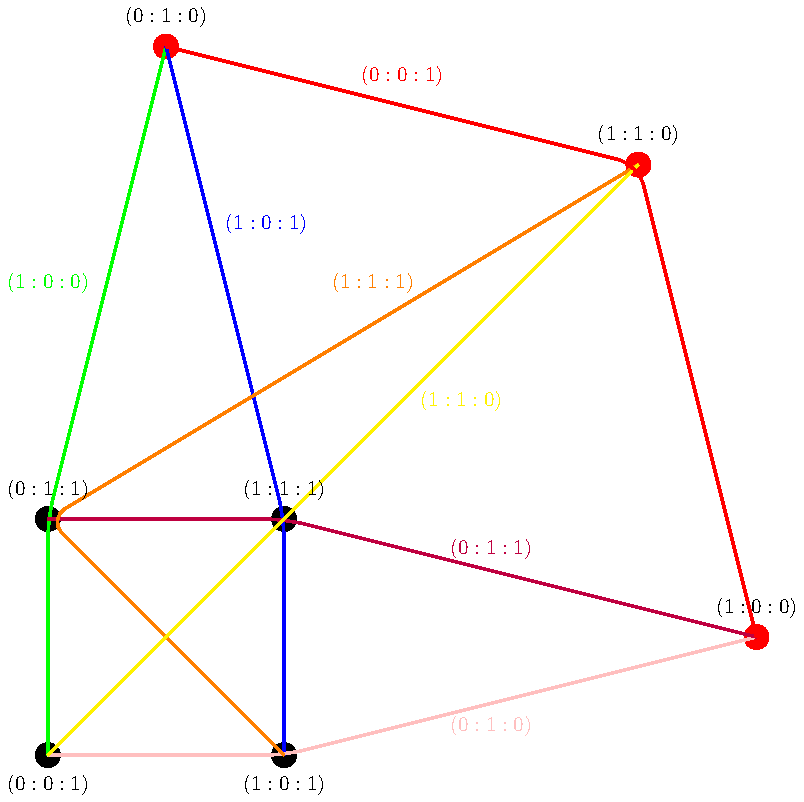
\includegraphics[scale=0.5]{droitestikz.pdf}
  \end{center}
\vspace{2\baselineskip}
\subsection{Plan de Hughes}
Sur certains plans projectifs, la propriété de Desargues n'est pas vérifiée, c'est le cas des plans de Hughes.\vspace{1\baselineskip}\\

Soit q un nombre premier impair (i.e. différent de 2).\\
Le plan de Hughes se base sur le corps fini $\mathbb{F}_{q^2}$ en utilisant toutefois une multiplication définie différemment de la multiplication ordinaire et non-commutative.\\
On construit $q**2-q+1$ droites d'équation $x + \alpha \circ y + z = 0$ que l'on notera $L(\alpha)$ comme on l'a fait pour la construction des plans projectifs sur des corps finis. On peut ensuite trouver pour chacune un ensemble de $q^2 + q + 1$ droites définies de la façon suivante à partir de n'importe quelle matrice A de taille 3*3 dont les éléments appartiennent à $\mathbb(F)_q$ et telle que $A^{q^2+q+1}=kI$ mais pas pour une puissance plus petite:
\begin{center}
 $ \{A^nL(\alpha) | 0 \leq n \leq q^2 + q\}$
\end{center}
\vspace{1\baselineskip}
J'ai fait puis ajouté la fonction HughesPlane dans le fichier $block\_design.py$ qui regroupe certaines fonctions comme $projective\_plane$ qui utilise la construction à partir des corps finis faite par la fonction $DesarguesianProjectivePlaneDesign$ aussi dans ce fichier.\\ Cette fonction a été acceptée pour être implémentée dans Sage, ce qui a été fait dans la version beta3 de Sage 6.8 le 4 Juin.
\newpage
Cette fonction s'appuie sur deux autres fonctions dont une fabrique une matrice A comme expliqué ci-dessus et une autre qui normalise les points ( $(a,b,c)k = (a,b,c)$ ). La fonction principale $HughesPlane$ suit la méthode de construction expliquée précédemment.
\begin{sageverbatim}
 sage: H = designs.HughesPlane(9)
 sage: H
 (91,10,1)-Balanced Incomplete Block Design
\end{sageverbatim}
Les \textit{Balanced Incomplete Block Design} sont des designs combinatoires ou plus précisemment des structures d'incidence avec 3 paramètres, ici $(91, 10, 1)$, ce qui signifie qu'il y a dans cette structure 91 points, 10 points par droite et par deux points passent une droite, ce qui correspond parfaitement à ce que l'on a vu sur les plans projectifs (ici $k=9$ : $k+1=10$ et $k^2+k+1=91$).\\
Nous allons montrer que ce plan de Hughes n'est pas desarguesien. J'ai recherché avec un algorithme les points qui nous permettraient de montrer ceci, je prends donc ici les triangles $(0,1,10)$ et $(57, 70, 59)$. Nous allons montrer que les intersection $D_{0,1} \cap D_{57,70}$, $D_{1,10} \cap D_{70,59}$ et $D_{10,0} \cap D_{59,57}$ sont alignées tandis que les droites $D_{0,70}$, $D_{1,59}$ et $D_{10,57}$ ne s'intersectent pas en un seul point.
\begin{sageverbatim}
 sage: blocks = H.blocks()
 sage: blocks[:3]
 [[0, 1, 2, 3, 4, 5, 6, 7, 8, 81],
 [0, 9, 18, 27, 36, 45, 54, 63, 72, 90],
 [0, 10, 20, 30, 40, 50, 60, 70, 80, 89],
 [0, 11, 23, 31, 43, 51, 55, 71, 75, 88]]
\end{sageverbatim}
La méthode $.blocks()$ depuis une structure d'incidence permet de nous donner la liste des droites. Il y en a 91 donc je me contente d'en afficher 4.
\begin{sageverbatim}
 line = lambda p,q: (b for b in blocks if p in b and q in b).next()
\end{sageverbatim}
On crée une fonction $line$ qui à p,q associe la droite qui passe par p et q.
\begin{sageverbatim}
 sage: set(line(0, 1)).intersection(line(57, 70))
 {2}
 sage: set(line(1, 10)).intersection(line(70, 59))
 {73}
 sage: set(line(10, 0)).intersection(line(59, 57))
 {60}
\end{sageverbatim}
$line$ nous renvoie une liste (une droite est une liste de points). Nous cherchons à avoir l'intersection de deux listes, ce qui n'est pas possible. Grâce à la fonction $set$, on transforme une des deux listes en un ensemble que l'on peut maintenant utiliser pour trouver l'intersection avec une liste. Nos intersections sont donc les points 2, 73 et 60.
\begin{sageverbatim}
 sage: line(2, 73) == line(73, 60)
 True
\end{sageverbatim}
La droite passant par 2 et 73 est la-même que celle passant par 73 et 60, on a donc bien que les points 2, 60 et 73 sont alignés.
\begin{sageverbatim}
 sage: set(line(0, 57)).intersection(line(1, 70))
 {82}
 sage: set(line(1, 70)).intersection(line(10, 59))
 {72}
\end{sageverbatim}
Les droites $D_{0,70}$, $D_{1,59}$ et $D_{10,57}$ ne sont pas concourrantes.
Plus concrètement voilà ce qu'il se passe dans ce plan de Hughes:
\begin{center}
  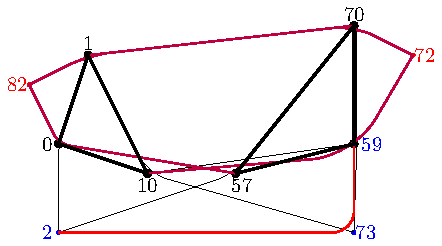
\includegraphics[scale=1.5]{Hughestikz.pdf}
\end{center}
72 et 82 devraient être le même point si le théorème de Desargues s'appliquait ici.

\newpage

\section{Le logiciel Sage}
\subsection{Présentation}
\textit{SageMath} est un logiciel libre de mathématiques qui se veut être une alternative libre à Matlab, Maple...\vspace{1\baselineskip}\\

Il est basé sur le langage Python et combine plusieurs dizaines de programmes libres dans une interface commune.\\
SageMath permet de travailler sur une vaste gamme de Mathématiques. Au cours de ce stage je ne travaille que dans la partie combinatoire de Sage et plus précisemment dans les designs combinatoires.
\vspace{3\baselineskip}
\begin{center}
  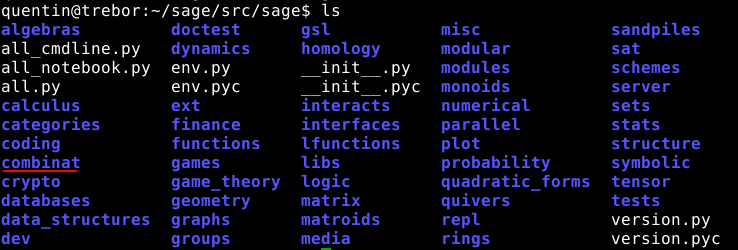
\includegraphics[scale=0.6]{matieres.jpg}
\end{center}
\vspace{3\baselineskip}
Sage étant un logiciel libre, le code source est entièrement accessible et modifiable. Il est en constante évolution, plusieurs mises à jours stables sortent par année. Le développement de Sage (les implémentations de nouvelles fonctions, de nouvelles classes, les corrections de bugs) se fait par tou-te-s les utilisat-rice-teurs qui proposent via le Trac de Sage (application web Open Source de gestion de projets) leur apport qui est ensuite discuté et éventuellement validé.
\newpage
\subsection*{Mon travail sur Sage}
\begin{itemize}
\item Ajout de la fonction \textit{is\_projective\_plane} dans \textit{incidence\_structure.py}\\
  Ticket \#18439 :\\
  \begin{sageverbatim}
 http://trac.sagemath.org/ticket/18439
  \end{sageverbatim}
 Fonction modifiée et placée dans \textit{design\_pyx.pyx} après discussion sur le trac. Correction d'une faute dans la référence d'une erreur dans le code d'une autre fonction repérée pendant la discussion. Fonction dans Sage depuis le 4 Juin avec la beta3 de Sage6.8.\vspace{1\baselineskip}\\
\item Ajout de la fonction \textit{HughesPlane} dans \textit{block\_design.py}\\
  Ticket \#18527 :\\
  \begin{sageverbatim}
 http://trac.sagemath.org/ticket/18527
    \end{sageverbatim}
  Fonction acceptée et dans Sage depuis le 4 Juin avec la beta3 de Sage6.8.\vspace{1\baselineskip}\\
\item Ajout des méthodes \textit{arc} et \textit{blocking\_set} pour la classe \textit{BalancedIncompleteBlockDesign} dans \textit{bibd.py}\\
  Ticket \#18608 :\\
\begin{sageverbatim}
 http://trac.sagemath.org/ticket/18608
\end{sageverbatim}
\vspace{1\baselineskip}
  Encore en discussion sur le trac à la remise du rapport de stage.\\
\end{itemize}  

\subsection{Ajout d'une fonction dans Sage}
Je prendrais ici l'exemple de la fonction \textit{HughesPlane}.\vspace{1\baselineskip}\\
Après avoir codé une nouvelle fonction en langage Python, il est d'abord nécessaire de la tester avec le logiciel sage:
\begin{center}
  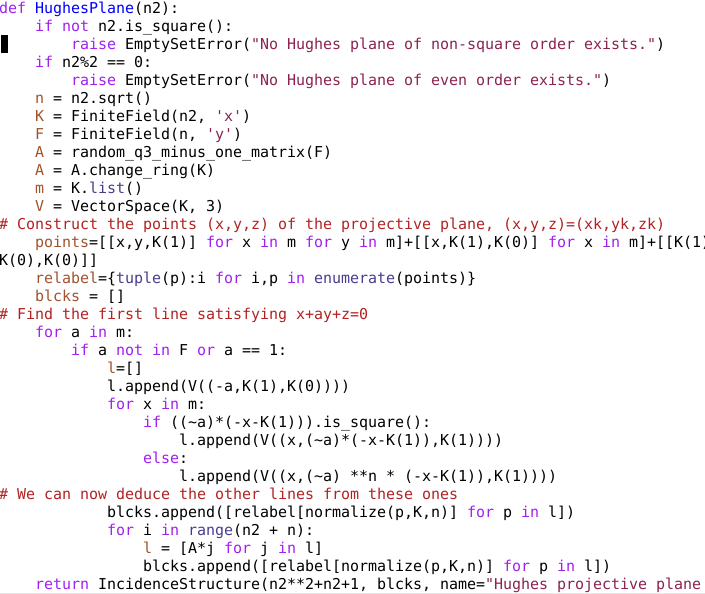
\includegraphics[scale=0.7]{hughes.png}\\
  La fonction dans le fichier hughes.py
\end{center}
\vspace{1\baselineskip}
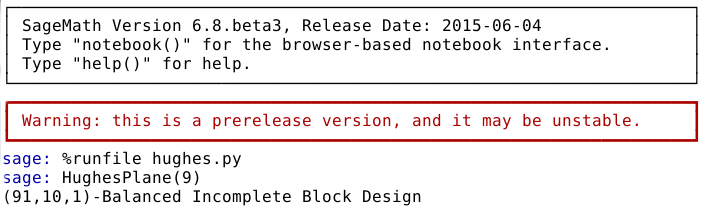
\includegraphics[scale=0.7]{hughessage.png}\vspace{1\baselineskip}\\
Si il n'y a pas de soucis de fonctionnement, on peut alors copier notre fonction dans le code de Sage. Nous allons ici le mettre dans le fichier $block\_design.py$ dans le dossier sage/src/sage/combinat/designs/.
\newpage
Toute fonction de Sage doit être accompagnée d'une documentation avec un format bien défini. On peut ainsi construire le manuel de référence ensuite.\\
\begin{center}
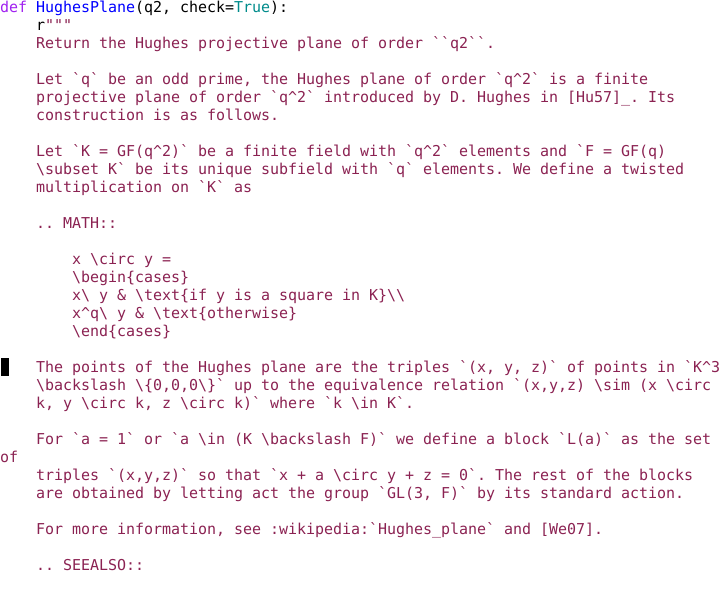
\includegraphics[scale=0.5]{hughesdoc.png}\\
  Extrait de la documentation écrite dans $block\_design.py$\vspace{1\baselineskip}

  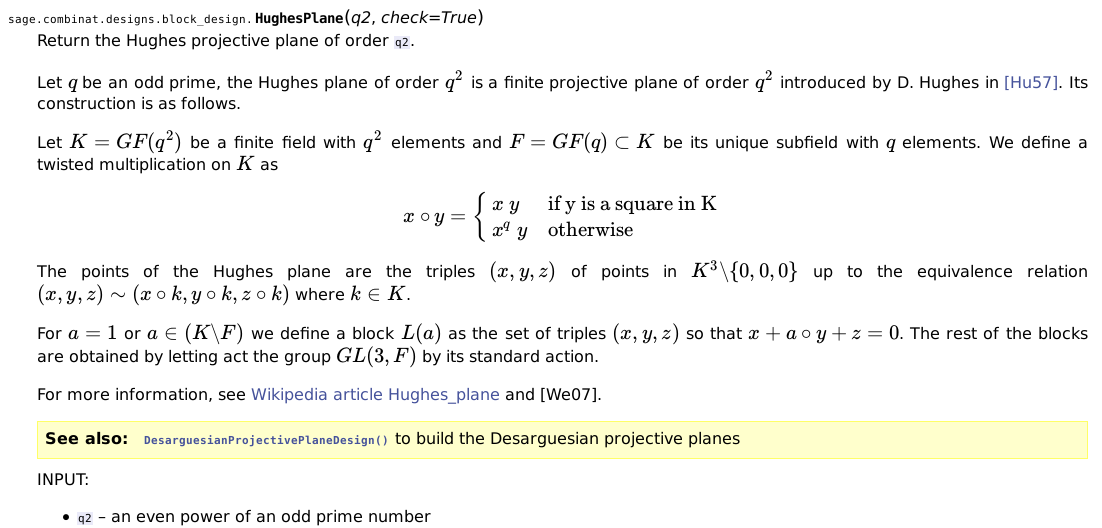
\includegraphics[scale=0.5]{hughesdocmanual.png}
  Extrait de la documentation dans le manuel de référence
\end{center}
Cette documentation doit contenir une phrase courte de description de la fonction. Ensuite une description plus complète peut être écrite. Si les sorties et les entrées de la fonction ne sont pas évidentes, il faut ajouer un bloc INPUT et un bloc OUTPUT. Comme on le voit ici, il est possible d'écrire des formules en LaTEX dans un bloc MATH, de faire des références à un article wikipedia, un site, une autre fonction. La documentation doit aussi contenir des exemples d'utilisation de la fonction et éventuellement des tests.\\
\newpage
On peut maintenant construire la librairie de Sage en utilisant la commande \textit{sage -b} dans un terminal. Les modifications qu'on a apporté seront maintenant prises en compte lorsqu'on utilisera Sage. Il est souvent nécessaire d'utiliser la commande \textit{sage -t block\_design.py} qui permet de tester les exemples et éventuellement d'afficher les erreurs dans le cas où il y en a. Par exemple:\vspace{1\baselineskip}\\
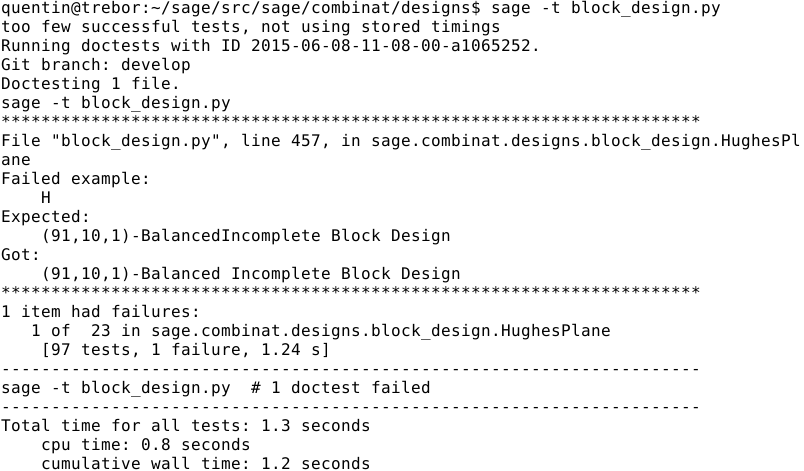
\includegraphics[scale=0.6]{hugheserror.png}\vspace{1\baselineskip}\\
Il ne reste alors plus qu'à construire le manuel de référence avec la commande \textit{sage -docbuild} afin de vérifier là aussi que la compilation de la documentation écrite dans le fichier donne ce que l'on attendait.



\newpage
\subsection{La programmation linéaire}
  Un programme linéaire est un système d’équations linéaires dont on cherche une solution optimale. Résoudre un programme linéaire revient à trouver la valeur des variables qui maximise (ou minimise) une fonction objectif, tout en satisfaisant un système de contraintes.\vspace{1\baselineskip}\\
\textbf{Exemple}\\
  On cherche à maximiser $x + y + 3z$ tel que : \\
  $x + 2y \leq 4$\\
  $5z - y \leq 8$\\
  La solution ici est $x = 4, y = 0, z = 1.6$\vspace{1\baselineskip}\\
La programmation linéaire lorsqu'on l'utilise est pour nous une boite noire. Le fonctionnement de cette boite est compliqué et bien optimisé. Il nous évite la programmation de grandes boucles très couteuses et bien trop longues dès que l'on a suffisamment de variables. Ces boucles testeraient alors toutes les combinaisons pour chercher celle qui maximise la fonction objectif (et encore, cette méthode n'est pas vraiment possible sur les réels ou les entiers).\\
C'est un outil très utile pour les problèmes combinatoires.\vspace{1\baselineskip}\\
\textbf{Exemple}\\
  Pour comprendre les problèmes que l'on va chercher à résoudre, nous allons prendre un exemple plus concret:\vspace{1\baselineskip} \\
  On a devant nous notre sac à dos ayant une capacité limitée C que nous devons remplir avec des objets à notre disposition ayant chacun une utilité et un poids propres fixés entre 0 et 1. Par exemple, une gourde aura un poids de 0.39 pour une utilité de 0.85 tandis qu'un livre aura un poids de 0.35 pour une utilité de 0.26 (selon le livre).\vspace{1\baselineskip}\\
  Soit o un objet. On va introduire une variable binaire ``prendre'' telle que $prendre[o]=1$ si on prend o et 0 si on ne le prend pas. \\
  Notre objectif est d'avoir un sac rempli des objets les plus utiles, on veut donc maximiser:
  \begin{center}
    $\sum_o utilit\acute{e}[o] * prendre[o]$
  \end{center}
  Cependant notre sac ayant une capacité limitée, il faut bien ajouter une contrainte sur le poids:
  \begin{center}
    $\sum_o poids[o] * prendre[o] \leq C$
  \end{center}
  Grâce à la programmation linéaire, on pourra donc savoir quelle combinaison d'objets pouvant rentrer dans notre sac est la plus utile.
\newpage
\subsubsection*{Dans Sage}
Nous avons dans Sage la classe $MixedIntegerLinearProgram$ qui représente les programmes linéaires que nous avons vu.
Nous allons résoudre le premier exemple avec Sage:
\begin{sageverbatim}
sage: p = MixedIntegerLinearProgram()
sage: x, y, z = p['x'], p['y'], p['z']    # on definit les variables
sage: p.set_objective( x + y + 3*z )
sage: p.add_constraint( x + 2*y <= 4 )
sage: p.add_constraint ( 5*z - y <= 8 )
sage: p.solve()         # sage nous retourne la valeur maximale de l'objectif
8.8
sage: p.get_values(x,y,z)    # on peut demander les valeurs des variables
[4.0, 0.0, 1.6]
\end{sageverbatim}
\subsubsection*{Les fonctions arc et blocking\_set}
La programmation linéaire va nous être utile pour trouver les arcs et les blocking set dans les plans projectifs finis. En effet, en associant une valeur binaire à chaque point du plan : 1 si on prend le point dans l'ensemble recherché, 0 sinon.\\
A partir de cet énoncé, on peut faire un programme pour trouver un arc de cardinalité maximale ou un \textit{committee} (un \textit{blocking set} de cardinalité minimale).

Soit s une structure d'incidence :

\begin{lstlisting}
from sage.numerical.mip import MIPSolverException
from sage.categories.sets_cat import EmptySetError
          
def arc(s):   
    p = MixedIntegerLinearProgram()
    b = p.new_variable(binary=True)
# La variable b comme une variable binaire #

    p.set_objective(p.sum(b[v] for v in s._points))
# Notre objectif est le nombre de points dans notre arc #

    for i in s._blocks:
        p.add_constraint(p.sum(b[k] for k in i) <= 2)
# On ne doit avoir au maximum que deux points d'un arc sur une ligne #
        
    try:
        p.solve()
        r = p.get_values(b)
        return [i for (i,j) in r.items() if j == 1]
    except MIPSolverException:
        raise EmptySetError('There is  no arc in this incidence structure.')
\end{lstlisting}
La méthode \textbf{try}/\textbf{except} permet de tester un énoncé sans craindre les erreurs qui pourraient arrêter le programme. Ici, si \textit{p.solve()} fonctionne (i.e. on trouve des solutions à ce problème linéaire), alors on renvoie les résultats. Si l'erreur MIPSolverException est générée par le solveur (i.e. il ne trouve pas de solutions), on choisit alors de renvoyer l'erreur EmptySetError qui correspond aux cas où l'ensemble des solutions est vide.

\begin{lstlisting}
def blocking_set(s):
    p=MixedIntegerLinearProgram(maximization=False)
# On minimise plutot que maximise #

    b=p.new_variable(binary=True)
    p.set_objective(p.sum(b[v] for v in s._points))
    for i in s._blocks:
        p.add_constraint(p.sum(b[k] for k in i)>=1)
# Chaque ligne doit etre intersectee #

        p.add_constraint(p.sum(b[k] for k in i)<=len(i)-1)
# Aucune ligne ne doit etre contenue entiere #
        
    try:
        p.solve()
        r=p.get_values(b)
        return [i for (i,j) in r.items() if j==1]
    except MIPSolverException :
        raise EmptySetError('There is no blocking set in this
    incidence structure')  
\end{lstlisting}
\vspace{1\baselineskip}
Les fonctions $blocking\_set$ et $arc$ ont été proposées sur le trac de Sage. A ce jour, elles sont encore en discussion sur le ticket $\#18608$.\vspace{3\baselineskip}\\

\textbf{Remarque}\\
Ces programmes pour trouver les arcs et les blocking set des plans projectifs sont efficaces pour les plans de petite taille mais deviennent trop lents pour des plans d'ordre suffisamment grands. Ceci est du au MIPSolver qui n'est pas assez efficace lorsque le nombre de variables est trop grand (étant donné que ce nombre évolue en $k^2 + k + 1$ par rapport à l'ordre).\\
J'ai suivi la veille de la remise de ce rapport un atelier sur les solveurs SATavec Laurent Simon, chercheur au LaBRI et professeur à l'Enseirb-Matmeca. Ces solveurs travaillent sur des variables booléennes (True / False) et cherchent quelle doit être la valeur de ces variables pour satisfaire une formule de logique propositionnelle (une formule utilisant les variables et les connecteurs 'et', 'ou', 'non', 'implique', 'équivaut'). Les solveurs SAT sont plus efficaces que les solveurs MIP.
\newpage
\section*{Le logiciel Git}
Bien que le logiciel Git passe au second plan, ce logiciel m'a été utile pendant toute la durée de ce stage.\\
Git est un logiciel de gestion de versions décentralisé. C'est donc un logiciel utilisés pour le développement et celui-ci ne se fait pas sur un serveur centralisé, chaque personne développe depuis son propre ``dépot''. Git est particulièrement utile lorsque plusieurs personnes travaillent sur un même projet pour ne pas se perdre dans les modifications des autres ou les écraser, etc... Même seul-e, git permet de garder un historique et les sauvegardes des anciennes versions du code source sur lequel on travaille.\\
Jusqu'ici, il ne s'agit que d'un logiciel de gestion de sauvegardes. Git retient en plus qui a fait telle modification et pourquoi (la personne écrit une courte phrase pour chaque modification faite). On peut aussi fusionner deux versions d'un document en évitant d'écraser le travail de l'autre personne. En effet, git travaille sur plusieurs branches (versions parallèles d'un même projet).\vspace{1\baselineskip}\\

Sage utilise git pour son développement. Sage utilise les branches \textit{master} et \textit{develop}. \textit{master} est la branche de la dernière version stable du logiciel Sage. \textit{develop} est la branche de développement de Sage, elle se fusionne à la branche \textit{master} lors d'une nouvelle version stable. Enfin, pour chaque ticket sur le trac, une branche git est créée, si la modification est validée sur ce ticket, la branche est fusionnée à la branche \textit{develop}. Bien sûr, je n'ai pas les autorisations de faire moi-même ces fusions. On peut néanmoins récupérer les versions de ces branches et accéder à tout l'historique depuis les premières étapes de création du logiciel. \vspace{2\baselineskip}\\
\begin{center}
  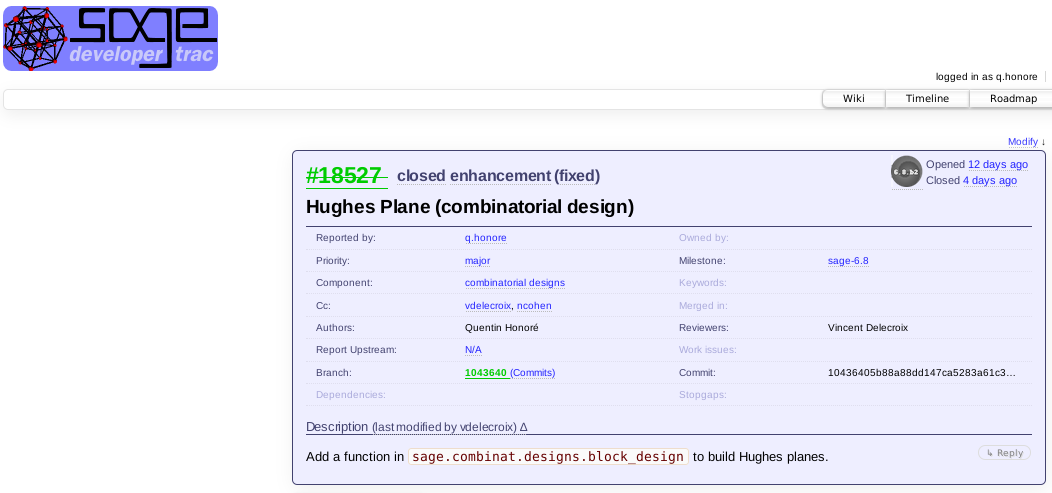
\includegraphics[scale=0.5]{trac.png}\\
  Interface trac pour le développement de Sage
\end{center}
\vspace{1\baselineskip}
En plus de l'utiliser pour participer au développement de Sage, git m'a permis de communiquer plus facilement tous les fichiers nécessaires à mon maitre de stage via GitHub qui est une sorte de réseau social pour développeurs sur lequel chaque personne peut poster son projet. Ainsi, j'ai pu envoyer et mettre à jour sur ce site tous les fichiers que je créais ou modifiais. A partir de ces fichiers, on peut me proposer des modifications sur une nouvelle branche que je peux choisir de fusionner avec la mienne ou encore récupérer les fichiers que j'ai mis en ligne.


\newpage
\thispagestyle{empty}

\section*{Annexes}

\includegraphics[scale=0.43]{dobble1.png}
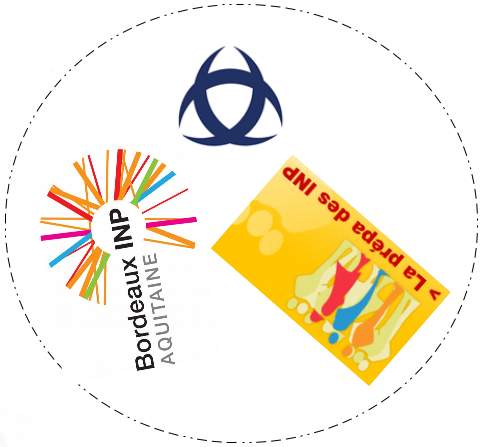
\includegraphics[scale=0.43]{dobble2.png}\\
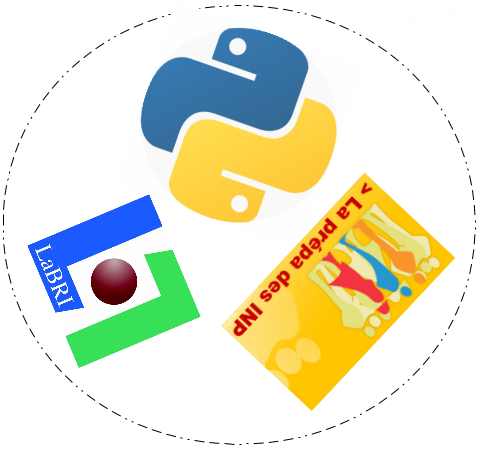
\includegraphics[scale=0.43]{dobble3.png}

\includegraphics[scale=0.43]{dobble4.png}\\
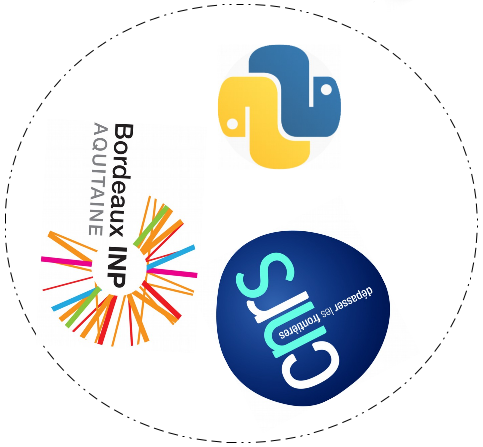
\includegraphics[scale=0.43]{dobble5.png}

\includegraphics[scale=0.43]{dobble6.png}\\

\includegraphics[scale=0.43]{dobble7.png}
\end{document}
